\documentclass[a4]{article}
\usepackage{geometry}
\geometry{a4paper,left=2cm,right=3cm, top=2cm, bottom=2cm} 
%\usepackage[austrian]{babel}
\renewcommand{\familydefault}{\sfdefault}
\usepackage{amsfonts,latexsym,amssymb,graphicx}
\usepackage{subfigure,epsfig,epstopdf}
%\usepackage{pdfsync}
\usepackage[utf8]{inputenc}
%\usepackage[T1]{fontenc}
\usepackage{booktabs} % For professional looking tables
\usepackage{multirow}
\usepackage{amsmath}

\usepackage[section]{placeins}

\title{\bf 183.605 \\ Machine Learning for Visual Computing \\ Assignment 2}
\author{Group 12: \\
	Hanna Huber (0925230) \\ Lena Trautmann (1526567) \\ Elisabeth Wetzer (0726681)}
\date{\today}


\begin{document}
\maketitle
\noindent

\section{Assignment 2}
\subsection{The dual optimization problem}

\noindent {\bf Tasks:}
\begin{itemize}
\item Generate a suitable training set of linearly separable data
\end{itemize}
%todo answer

\begin{itemize}
\item Plot the input vectors in $\mathbb{R}^2$ and visualize corresponding target values (e.g. by using color). 
\end{itemize}
%todo answer (das was noch steht ist von assignment 1)
\begin{figure}[!h]
	\begin{center}
		\centering
%		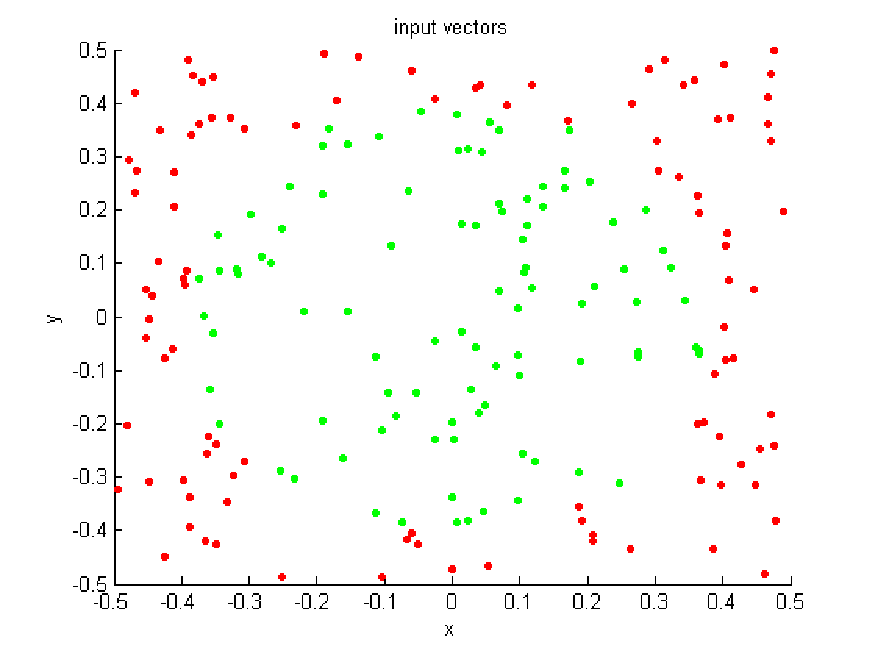
\includegraphics[width=6cm]{../figures/inputVectors.pdf}
	\end{center}	
	\caption{Plot of the input vectors with the target value visualized by colour.}
	\label{fig:inputVectors}
\end{figure}
Figure~\ref{fig:inputVectors} shows the input vectors.

\begin{itemize}
\item Visualize the support vectors and plot the decision boundary.
\end{itemize}
%todo answer (das was noch steht ist von assignment 1)
\begin{figure}[!h]
	\begin{center}
		\centering
%		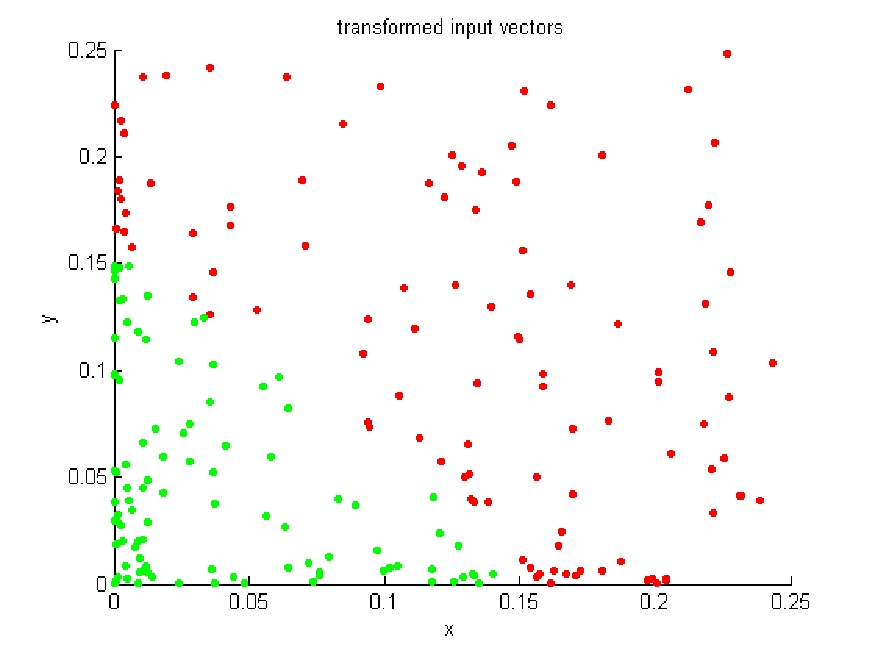
\includegraphics[width=6cm]{../figures/transformedInputVectors.pdf}
	\end{center}
	\caption{Plot of the transformed input vectors with the target value visualized by colour.}
	\label{fig:transformedInputVectors}
\end{figure}
Figure~\ref{fig:transformedInputVectors} shows the transformed input vectors.

\subsection{The kernel trick}

\noindent {\bf Tasks:}
\begin{itemize}
\item Try different values for $\sigma$ (the RBF parameter).
\end{itemize}
\begin{figure}[h!]
\centering
	\subfigure[$\sigma=5$]{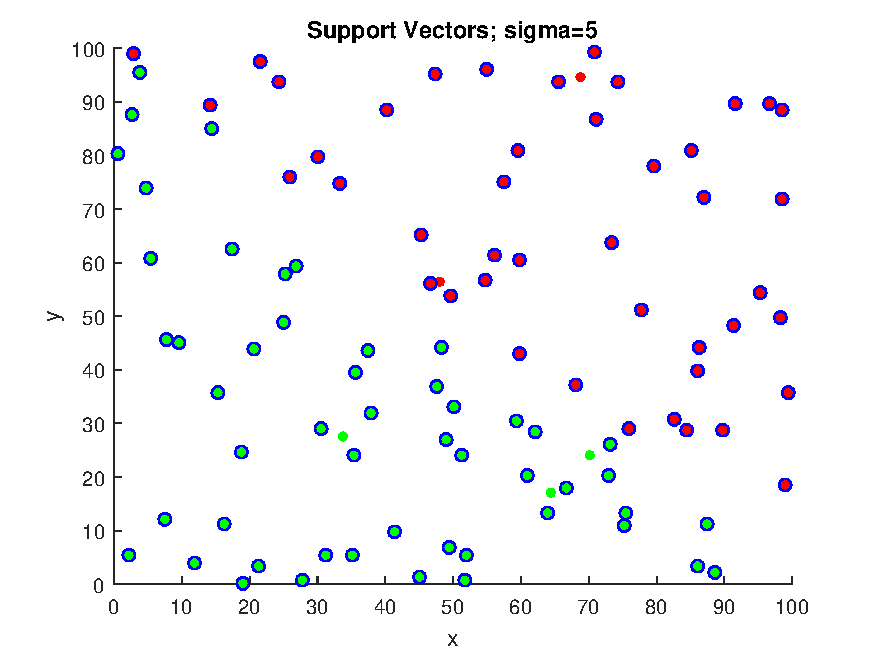
\includegraphics[width=5cm]{../figures/sv_kernel5.pdf}}
	\subfigure[$\sigma=15$]{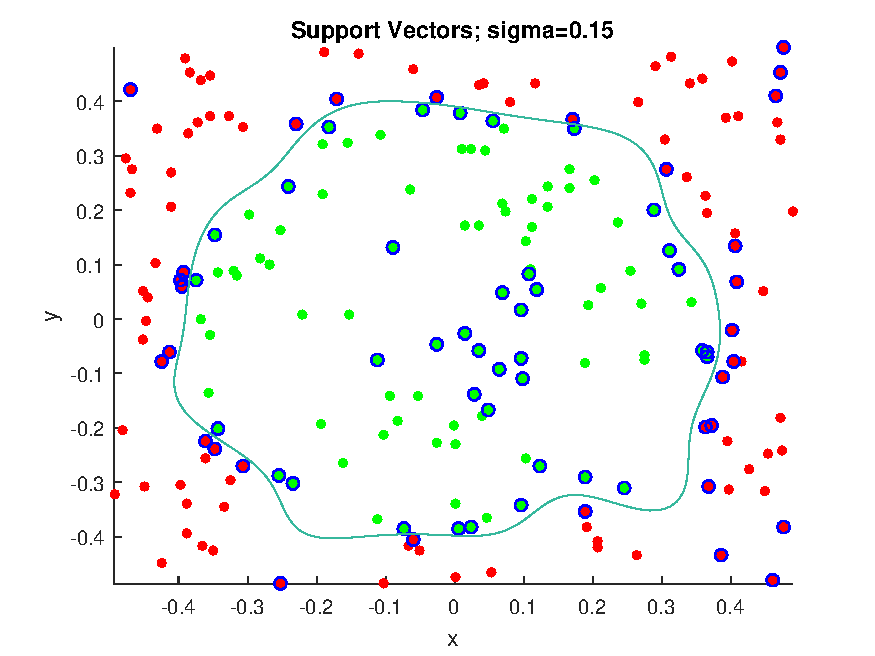
\includegraphics[width=5cm]{../figures/sv_kernel15.pdf}}
	\subfigure[$\sigma=25$]{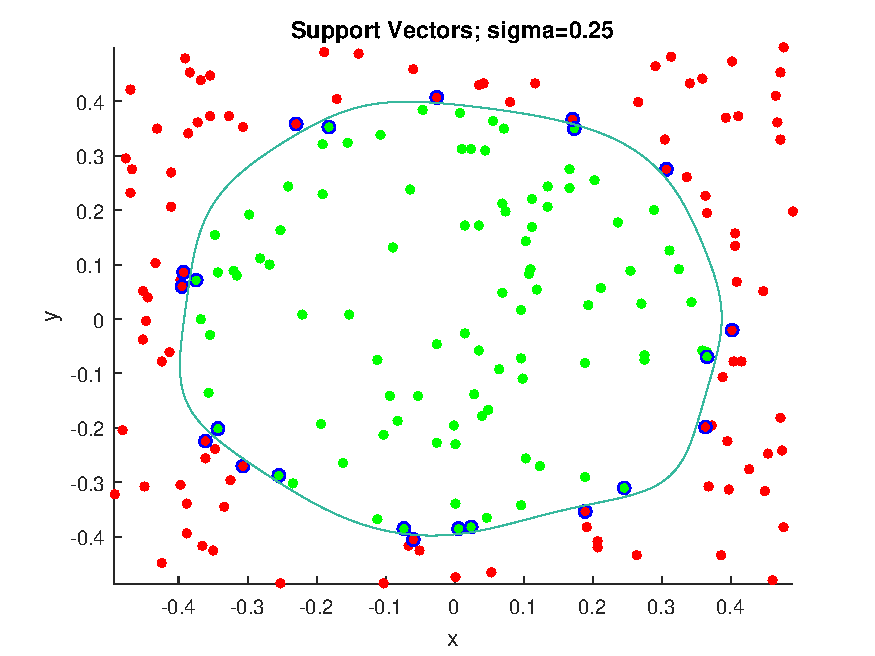
\includegraphics[width=5cm]{../figures/sv_kernel25.pdf}}
	\\
	\subfigure[$\sigma=35$]{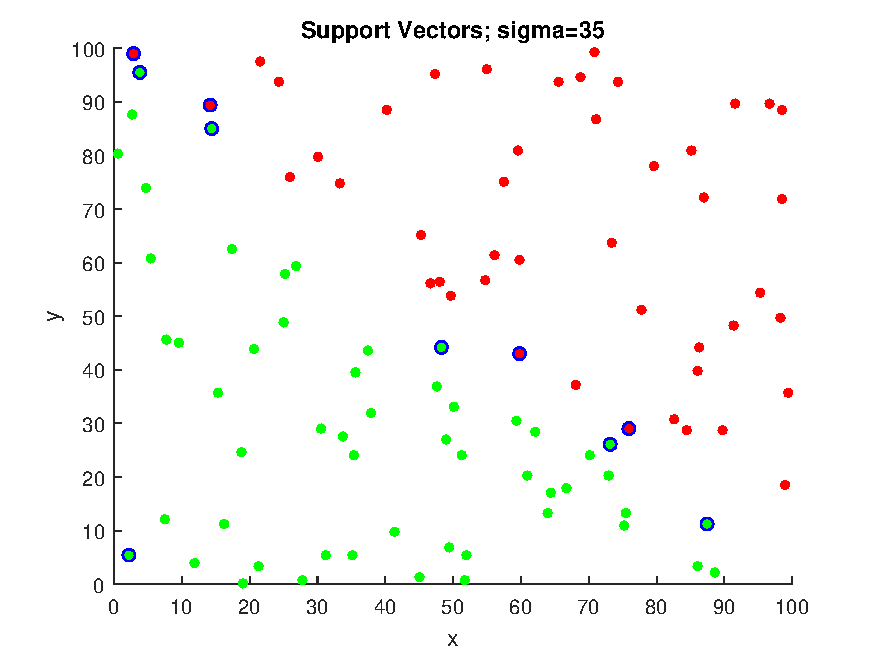
\includegraphics[width=5cm]{../figures/sv_kernel35.pdf}}
	\subfigure[$\sigma=45$]{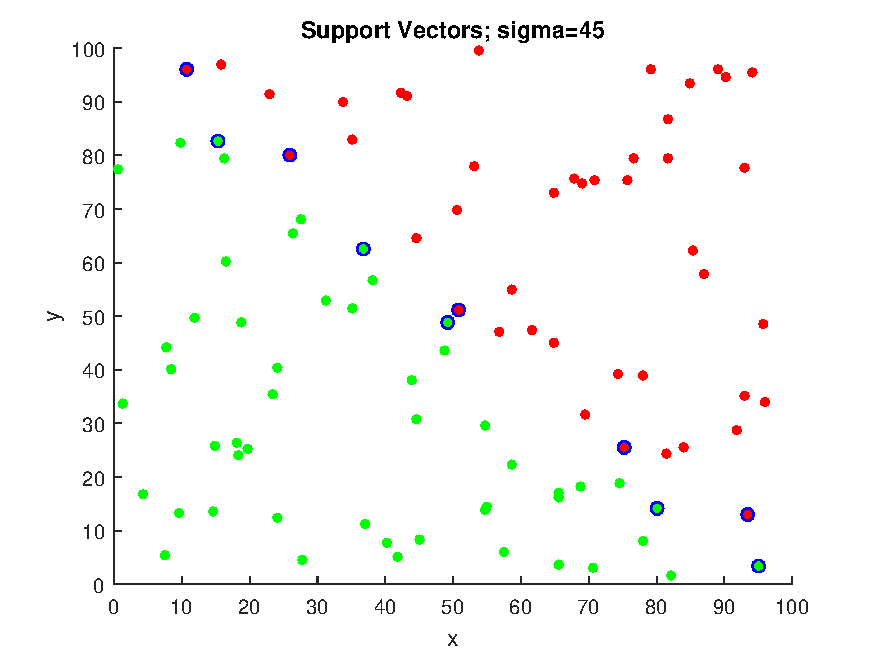
\includegraphics[width=5cm]{../figures/sv_kernel45.pdf}}
	\subfigure[$\sigma=55$]{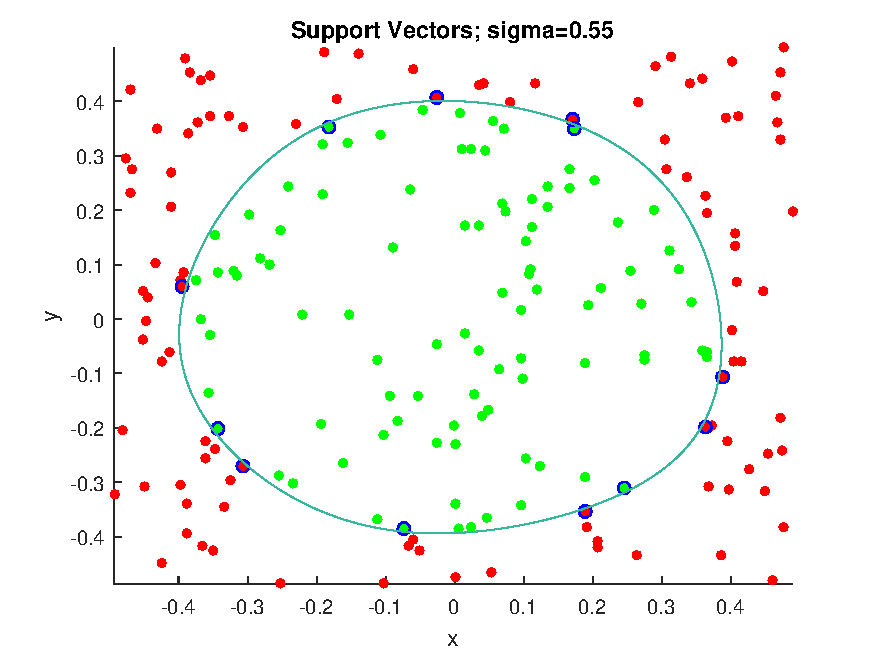
\includegraphics[width=5cm]{../figures/sv_kernel55.pdf}}
\caption{Support Vectors for different values of the RBF parameter $\sigma$.}
\label{fig:sv_kernel}
\end{figure}
The radial basis function kernel is defined by $K(x,y) = exp(-\frac{\|x-y\|^2}{\sigma^2})$.
The corresponding support vectors are shown in Figure~\ref{fig:sv_kernel} for different values of the RBF parameter $\sigma$. In the lecture notes about RBF-networks, we discussed a selection of $\sigma= 2*avgdist$, where $avgdist$ denotes the average distance of the centers. Having distances between the data points of approximately 10 units (or slightly more), $\sigma= 25$ is then selected.

\begin{itemize}
\item Generate a non-linearly separable training set, plot the data, visualize the support vectors and plot the decision boundary.
\end{itemize}
%todo answer (das was noch steht ist von assignment 1)
\begin{figure}[!h]
	\begin{center}
		\centering
%		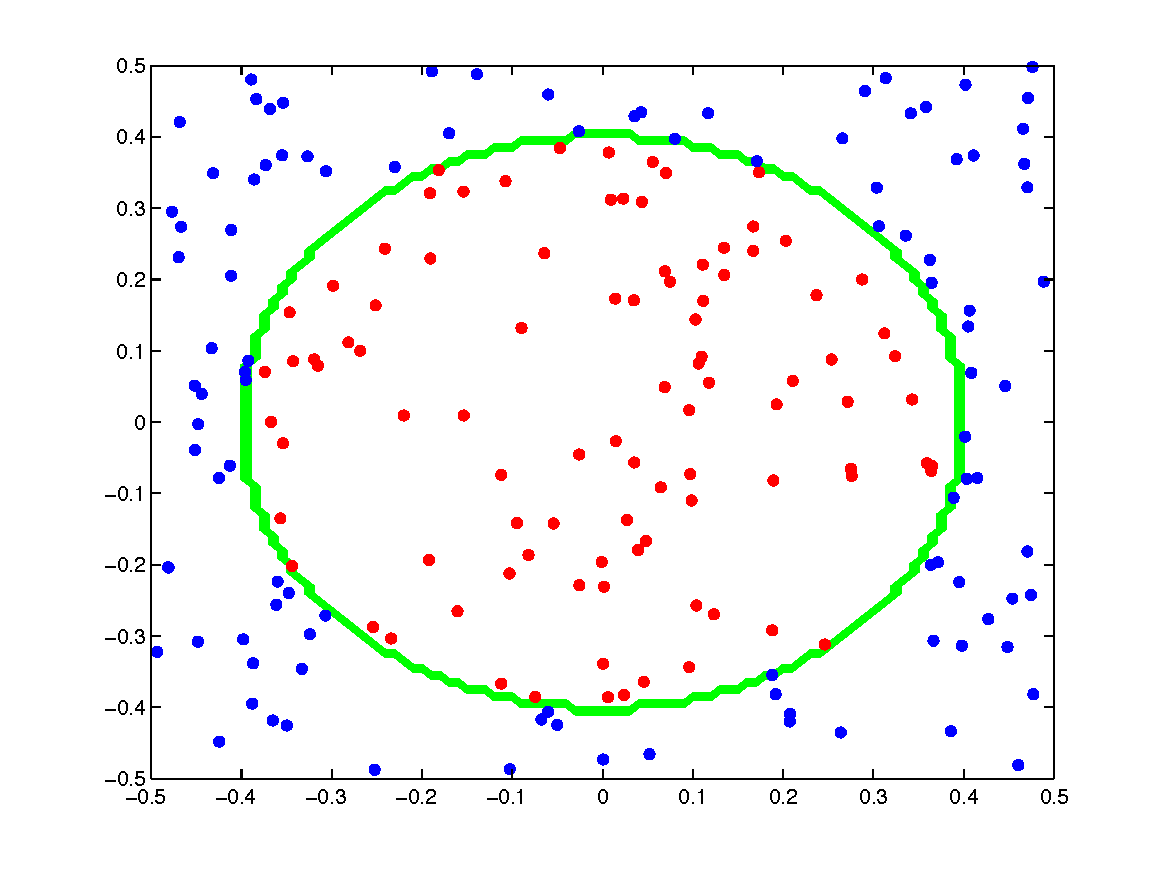
\includegraphics[width=6cm]{../figures/perceptron.pdf}
	\end{center}
	\caption{\label{fig:perceptron}Plot of the decision boundary in the original data space found by the perceptron (green curve) together with labelled data points.}
\end{figure}



%todo Variante für figure mit 3 subfigures.
%\begin{figure}[h!]
%\centering
%	\subfigure[]{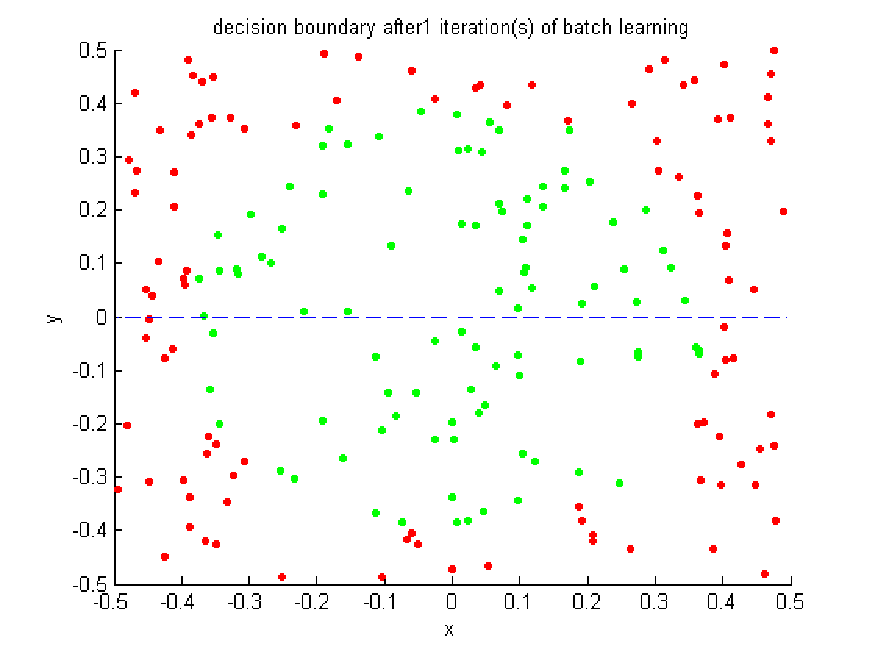
\includegraphics[width=5cm]{../figures/originalBatchIt1.pdf}}
%	\subfigure[]{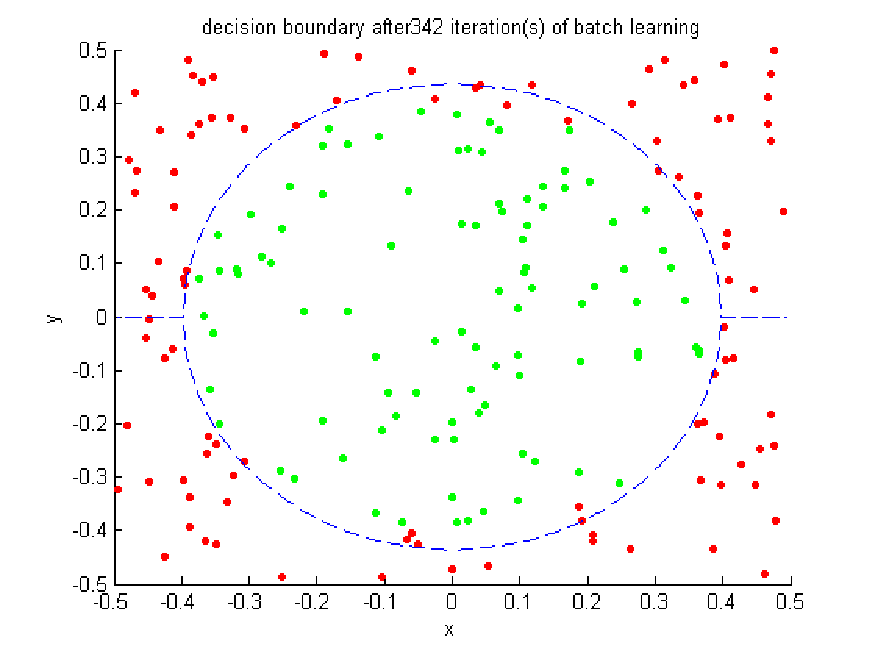
\includegraphics[width=5cm]{../figures/originalBatchIt342.pdf}}
%	\subfigure[]{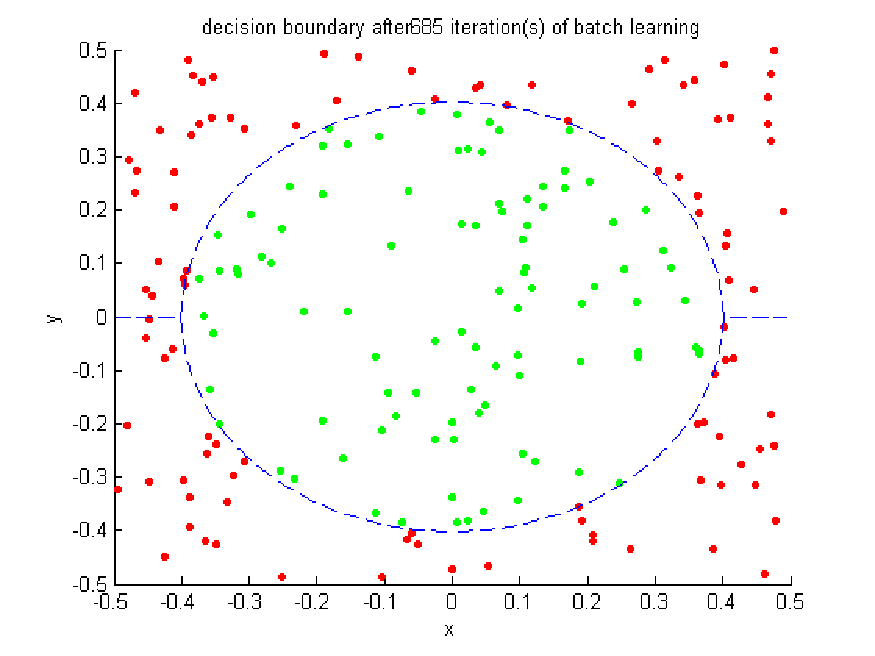
\includegraphics[width=5cm]{../figures/originalBatchIt685.pdf}}
%\caption{Perceptron decision boundary in the original data space at iterations \#1, \#342 and \#685 of batch learning.}
%\label{fig:origBA}
%\end{figure}


% \bibliography{lit}
% \bibliographystyle{unsrt}

\end{document}
